\vspace{-5mm}
\section{Experiments}
\label{sec:experiments}

\vspace{-1mm}
\subsection{Atari 100k benchmark}
\label{subsec:atari100k}
For comprehensive evaluation of \textsc{diamond} we use the established Atari 100k benchmark \citep{kaiser2019atari100k}, consisting of 26 games that test a wide range of agent capabilities. 
%These environments are visually diverse, with performance in many games depending on differences in the shapes, sizes and colors of objects. 
For each game, an agent is only allowed to take 100k actions in the environment, which is roughly equivalent to 2 hours of human gameplay, to learn to play the game before evaluation. 
As a reference, unconstrained Atari agents are usually trained for 50 million steps, a 500 fold increase in experience. 
We trained \textsc{diamond} from scratch for 5 random seeds on each game. 
Each run utilized around 12GB of VRAM and took approximately 2.9 days on a single Nvidia RTX 4090 (1.03 GPU years in total).

\begin{table*}[ht]
\resizebox{\textwidth}{!}{%
\begin{tabular}{@{}lllllll@{}}
\toprule
 &
   &
  \multicolumn{2}{c}{Lexical Diversity} &
  \multirow{2}{*}{\begin{tabular}[c]{@{}l@{}}Semantic \\ Diversity\end{tabular}} &
  \multirow{2}{*}{\begin{tabular}[c]{@{}l@{}}Syntactic \\ Diversity\end{tabular}} &
  \multirow{2}{*}{\begin{tabular}[c]{@{}l@{}}Compression \\ Ratio\end{tabular}} \\
                                                                           &            & Distinct-N & Self-BLEU &       &       &  \\ \midrule
\begin{tabular}[c]{@{}l@{}}Story\\ Generation\end{tabular}                 & Llama-3-8B & 0.298      & 0.372     & 0.441 & 0.897 &  \\
                                                                           & Mistral-7B & 0.261      & 0.368     & 0.443 & 0.890 &  \\
                                                                           & Qwen2-7B   &            &           &       &       &  \\
                                                                           & Falcon-7B  & 0.196      & 0.347     & 0.421 & 0.881 &  \\
                                                                           & Olmo1.7-7B &            &           &       &       &  \\
                                                                           & Gemma-7B   &            &           &       &       &  \\ \midrule
\begin{tabular}[c]{@{}l@{}}Dialogue \\  Generation\end{tabular} & Llama-3-8B & 0.426      & 0.396     & 0.467 & 0.882 &  \\
                                                                           & Mistral-7B & 0.420      & 0.409     & 0.458 & 0.852 &  \\
                                                                           & Qwen2-7B   & 0.483      & 0.461     & 0.463 & 0.854 &  \\
                                                                           & Falcon-7B  &            &           &       &       &  \\
                                                                           & Olmo1.7-7B &            &           &       &       &  \\
                                                                           & Gemma-7B   & 0.336      & 0.279     & 0.419 & 0.865 & 
\end{tabular}
}
\caption{Diversity results for the different tasks.}
\label{tab:results}
\end{table*}

We compare with other recent methods training an agent entirely within a world model in Table \ref{tab:atari_results_full}, including \textsc{storm} \citep{zhang2023storm}, DreamerV3 \citep{hafner2023dreamerv3}, \textsc{iris} \citep{iris2023}, \textsc{twm} \citep{robine2023transformer}, and SimPle \citep{kaiser2019atari100k}. A broader comparison to model-free and search-based methods, including \textsc{bbf} \citep{schwarzer2023bigger} and EfficientZero \citep{ye2021efficientzero}, the current best performing methods on this benchmark, is provided in Appendix \ref{app:additonal_baselines}. \textsc{bbf} and EfficientZero use techniques that are orthogonal and not directly comparable to our approach, such as using periodic network resets in combination with hyperparameter scheduling for \textsc{bbf}, and computationally expensive lookahead Monte-Carlo tree search for EfficientZero. Combining these additional components with our world model would be an interesting direction for future work.

\subsection{Results on the Atari 100k benchmark}
\label{subsec:results}

%%%%%%%%%%%%%%%%%%%%%%%
\begin{wrapfigure}[]{R}{0.50\linewidth}
\vspace{-15mm}
\begin{center}
\centerline{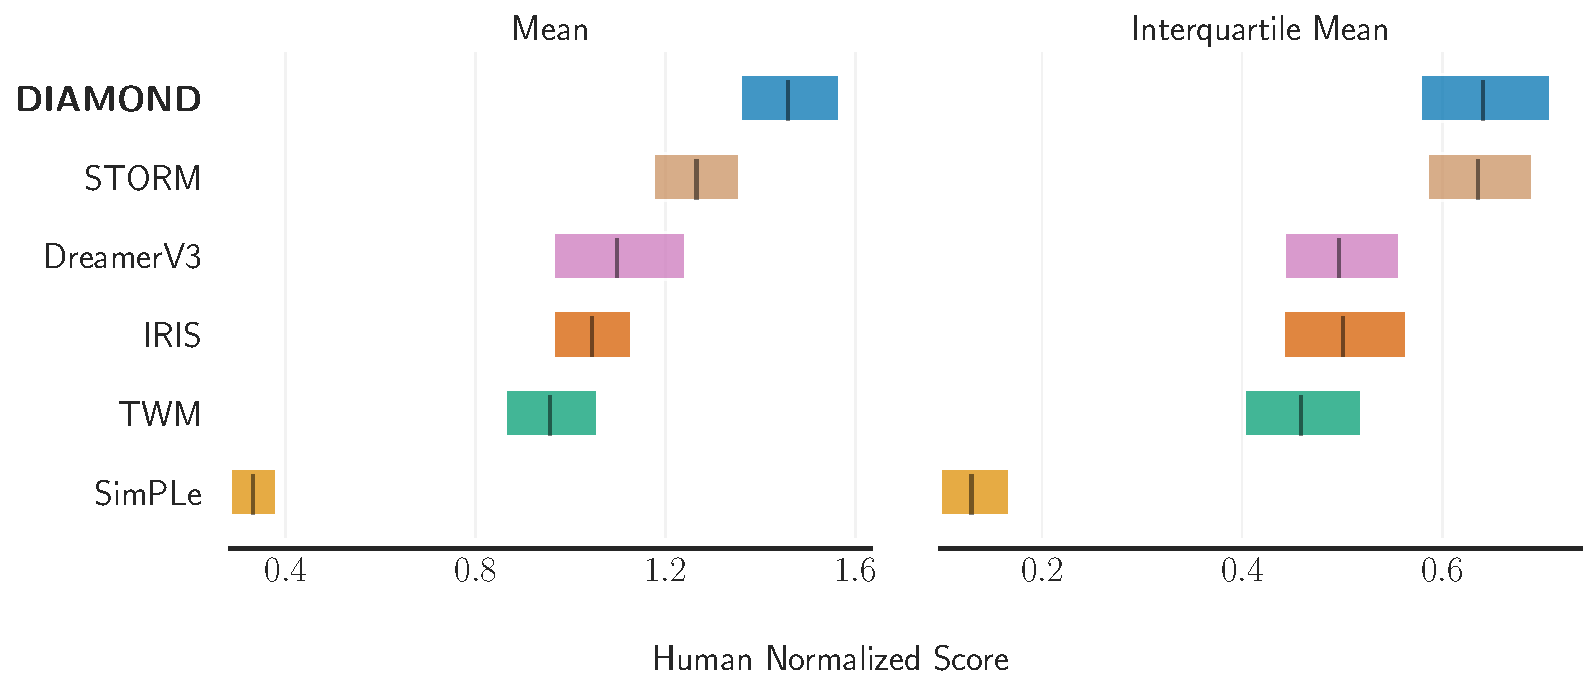
\includegraphics[width=\linewidth]{images/aggregates.pdf}}
\caption{Mean and interquartile mean human normalized scores. \textsc{diamond}, in blue, obtains a mean HNS of 1.46 and an IQM of 0.64.}
\label{fig:results_mean_IQM}
\end{center}
\vskip -15mm
\end{wrapfigure}
%%%%%%%%%%%%%%%%%%%%%%%


Table \ref{tab:atari_results_full} provides scores for all games, and the mean and interquartile mean (IQM) of human-normalized scores (HNS) \citep{dueling_networks}. Following the recommendations of \citet{agarwal2021deep} on the limitations of point estimates, we provide stratified bootstrap confidence intervals for the mean and IQM in Figure \ref{fig:results_mean_IQM}, as well as performance profiles and additional metrics in Appendix \ref{app:performance_profile}.

Our results demonstrate that \textsc{diamond} performs strongly across the benchmark, outperforming human players on 11 games, and achieving a superhuman mean HNS of 1.46, a new best among agents trained entirely within a world model. \textsc{diamond} also achieves an IQM on par with \textsc{storm}, and greater than all other baselines. We find that \textsc{diamond} performs particularly well on environments where capturing small details is important, such as \textit{Asterix}, \textit{Breakout} and \textit{Road Runner}. We provide further qualitative analysis of the visual quality of the world model in Section \ref{subsec:comparison_transformers}. 
